% !TeX root = ../../thesis.tex
\chapter{Model applications: mechanical loosening of mandibular plates}\label{ch:mandible}

\begin{shaded}
This chapter is based on a manuscript prepared to be submitted:\\
P. Ansoms, M. Barzegari, J. Vander Sloten, and L. Geris, ``Coupling biomechanical models of implants with biodegradation models: a case study for biodegradable mandibular bone fixation plates.''
\end{shaded}

\section*{Abstract}

In fracture fixation, biodegradable implant materials are an interesting alternative to conventional non-biodegradable materials as the latter require a second implant removal surgery to avoid long-term complications. In this study, we present an \textit{in silico} strategy to biodegradable metal implants focusing on mandibular fracture fixation plates of WE43 (Mg-alloy). The \textit{in silico} strategy is composed of an orchestrated interaction between three separate computational models. The first model simulated the mass loss of the degradable implant based on the chemistry of Mg biodegradation. A second model estimated the loading on the jaw plate in the physiological environment incorporating a phenomenological dynamic bone regeneration process. The third model characterized the mechanical behavior of the jaw plate and the influence of material degradation on the mechanical behavior. Multiple sensitivity analyses were performed on parameters related to choices regarding numerical implementation and parameter dependencies were implemented to guarantee robust and correct results. Different clinical scenarios were tested, related to the amount of screws used to fix the plate. The results showed a lower initial strength when more holes were left open, as well as a faster decrease over time in strength due to the increased area available for surface degradation. The combination of these three models facilitates the iterative design of patient-specific biodegradable fixation implants able to deliver the desired mechanical behavior tuned to the bone regeneration process.

\section{Introduction}

In clinical bone regeneration applications, biodegradable implants have gained in popularity over recent years. The main advantage of biodegradable implants over non-biodegradable implants is that no second surgery is needed to remove the implant after successful healing of the bone \cite{Zheng2014}. The removal of a non-biodegradable implant brings along an additional cost and risk of infection but might be necessary to avoid complications associated in the long term such as late thrombosis and chronic inflammation \cite{KChen}. Late thrombosis is the formation of blood cloths due to the presence of the metallic implant \cite{thrombosis}. Chronic inflammation is induced by the persistence of inflammatory stimuli, being the physical presence of the implanted biomaterial or the ability of the implant to slightly move at the implant site \cite{inflammation}. Permanent metallic implants also distort diagnostic images of the body \cite{Han}. Both in the short and long term, a biodegradable implant reduces stress shielding, which is the resorption of bone as a result of a reduction in perceived load. The reduction of stress shielding in the long term is obvious since the implant has disappeared in case of a biodegradable implant. Besides obvious reduction of long-term stress shielding due to the disappearance of the implant, there is also a reduction of stress shielding in the short term resulting from the fact that biodegradable metals often have a Young's modulus that is considerably lower than that of inert metals (e.g., 44.2 GPa for WE43 vs. 118 GPa for Ti6Al4V). The stress shielding effect is directly proportional to the E-modulus of the implant material.

The use of biodegradable metals to support tissue regeneration is mentioned in various sources, describing different materials and applications \cite{KChen,JChen,Yang}. The material of the implant determines the rate of degradation. The goal is to provide stable mechanical support at the early stage of the tissue healing process and then have the material gradually degrade with the restoration of the defect tissue \cite{Yang}. Fig. \ref{fig:rateofdeg} qualitatively shows the degradation rate of three common biomaterials (magnesium, zinc and iron) along with the healing rate of different tissues (hard, soft and vascular) as an illustration. By matching a material's degradation rate and a tissue's healing rate, a suitable material can be found for a specific application. Studying the change of mechanical support of implants due to biodegradation has certain complexities. This case-study aimed to gain insight into the change in mechanical behavior of a biodegradable mandibular fixation plate. In order to do this, three different models were combined: a biodegradation model to characterize the geometry change as a result of biodegradation, a model to characterize the loading on the jaw plate by considering the bone healing and a model to predict the mechanical behavior of the plate. These are schematically shown in Fig. \ref{fig:ModelCoupling}.

\begin{figure}[ht]
    \centering
    \medskip
    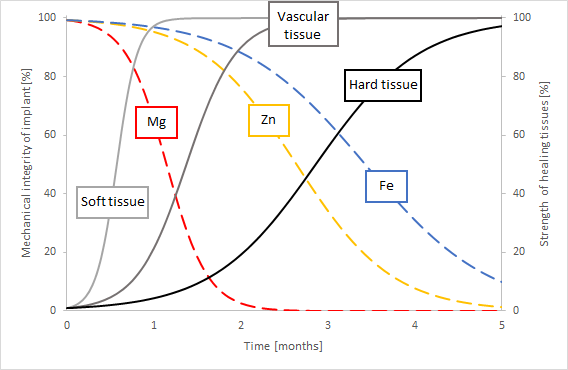
\includegraphics[width=0.86\textwidth]{MechanicalIntegrityTissueStrength.png}
    \caption[The change in mechanical integrity of the implant and tissue strength over time]{The change in mechanical integrity of the implant and tissue strength over time (adapted from \cite{KChen}).}
    \label{fig:rateofdeg}
\end{figure}

\begin{figure}[ht]
    \centering
    \medskip
    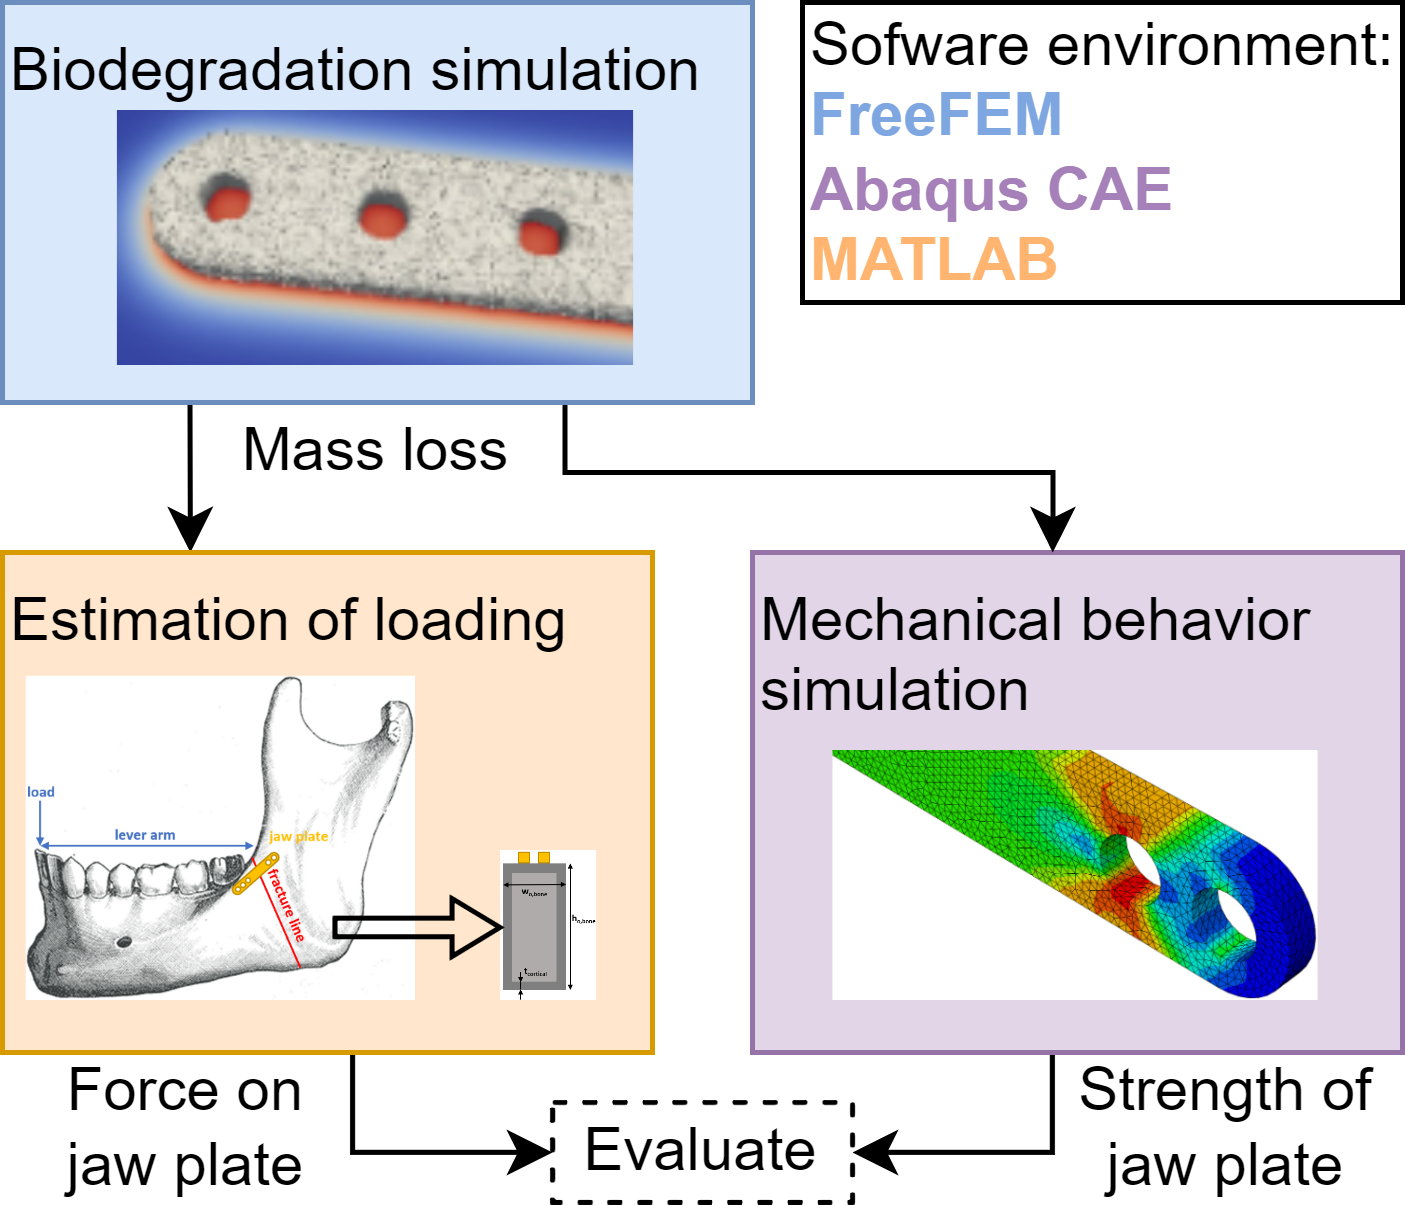
\includegraphics[width=0.8\textwidth]{ModelCoupling.png}
    \caption{Coupling of the models and indication of software used.}
    \label{fig:ModelCoupling}
\end{figure}

The mandible is the second most frequently fractured bone of the face and the tenth most frequently fractured bone of the body \cite{Bhavik}. Common causes for a mandible fracture are violence, car crashes and sports. It occurs more frequently in males than females and most often between the ages of 16 and 30. The weakest section of the mandible is the angle because there is an abrupt change in direction between the mandibular body and the ascending ramus, both in the sagittal and transverse planes, resulting in the involvement of the mandibular angle in up to 28.5\% of jaw fractures \cite{Levy}. The most common treatment of mandible fractures is with a mandibular fixation plate (further referred to as jaw plate) to stabilize the fracture and allow the healing process to take place. Though the plate is traditionally made of an inert implant material (e.g., titanium), biodegradable materials are explored to take advantage of the aforementioned benefits.

Computational models provide useful tools for designing plates and studying the implant-bone complex given their ability to simultaneously capture the mechanics and mechanisms of both the plate degradation and bone regeneration. Multiple studies reported in the literature focus on the biological processes after mandibular surgery, the design of the implant or its degradation separately and we refer to the reader to \cite{Vautrin2021}, \cite{Zheng2019}, \cite{Wu2020}, \cite{Boccaccio2008} and references within for an overview of those models. The combination of concurrent implant biodegradation and bone regeneration has been developed for long bones by Mehboob et al. \cite{Mehboob2015} and by Ma et al. \cite{Ma2018} while Vautrin et al. developed a combined biodegradation and tissue regeneration model in the context of orthognatic surgery \cite{Vautrin2021}. The bone healing algorithm of the latter was based on the model that Alierta et al. developed, but was generalized to be applicable to a larger fracture gap \cite{Alierta2013}. It modeled the growth of the contribution of cartilage and bone to the mechanical properties of each element within the fracture gap based on the principal element strains under physiological loading. The biodegradation algorithm was limited to being phenomenological to reduce the computational cost. It included only localized corrosion by incorporating a random pitting corrosion algorithm.

In this study, we started from an in-house developed biodegradation algorithm based on the chemistry of biodegradation of WE43 and combined it with a phenomenological bone regeneration algorithm. We used this combination of models to investigate the impact of biodegradation on the strength of the jaw plate. Additionally, we looked into the effect of the number of plate holes left unscrewed on the overall mechanics.

%%%%%%%%%%%%%%%%%%%%%%%%%%%%%%%%MATERIALS & METHODS

\section{Materials and methods}

\subsection{Mandibular plate and fixation}

The implant simulated in this study was a jaw plate, shown in Fig. \ref{fig:jawPlateDim}b (geometrical details discussed in section \ref{sec:FEA}). This jaw plate is placed on top of the manddibular body as shown in Fig. \ref{fig:MandibleForceLeverArm}. This technique of mandibular fracture fixation is called the ``miniplate fixation technique'', also known as ``semi-rigid'' or ``functionally adequate fixation''. The loading on the plate in this situation is purely tensile when a mastication load is applied. Different scenarios for its fixation used in clinical practice (different amounts of screws) were studied. Leaving holes open is a common occurrence due to proximity of the screw to the fracture line or it being located in a section of the bone that is simply too weak to carry the screw. Open holes are exposed to body fluids and hence might undergo a different degradation dynamic in that part of the plate.

\begin{figure}[h]
    \centering
    \medskip
    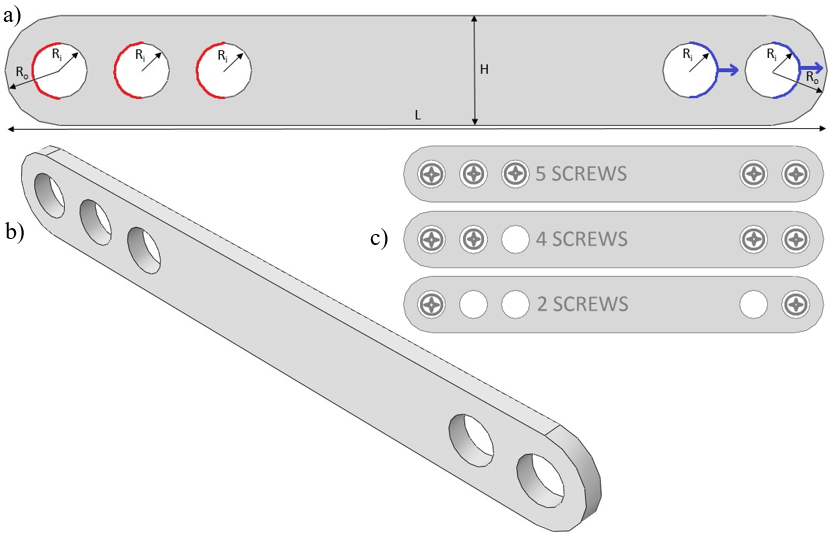
\includegraphics[width=\textwidth]{jawPlateDim.png}
    \caption[Indication of dimensions and screws placement on the jaw plate]{Jaw plate. a) Indication of inner (screw hole) radius $R_i$, outer radius $R_o$, height $H$ and length $L$ and boundary conditions for the five-screw case (red indicates the region where a fixed boundary condition is applied, blue indicates the region where a displacement boundary condition is applied, accompanied by arrows for direction). b) Different angle showing the depth of the jaw plate. c) Indication of screw placement in the three different cases.}
    \label{fig:jawPlateDim}
\end{figure}

\begin{figure}[h]
    \centering
    \medskip
    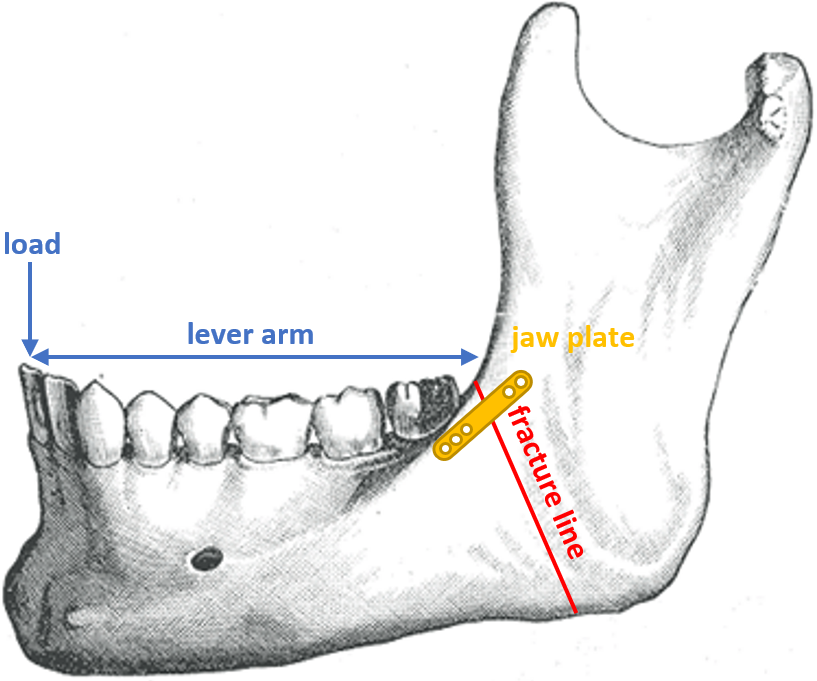
\includegraphics[width=0.7\textwidth]{MandibleForceLeverArm.PNG}
    \caption{Mandible with indication of fracture line, jaw plate, lever arm and load}
    \label{fig:MandibleForceLeverArm}
\end{figure}

%%%%%%%%%%%%

\subsection{Biodegradation simulation}
\label{sec:biodeg}

The biodegradation process was modeled as a set of partial differential equations (\gls{PDE}s), formulating the mass transfer phenomena as well as tracking the location of the surface of the implant during degradation as described in \cite{Barzegari2021} (Chapter \ref{ch:core}) and summarized below. For the mass transfer model, a system of time-dependent reaction-diffusion PDEs was derived from the underlying oxidation-reduction reactions in simulated body fluid (\gls{SBF}) solutions. This includes the oxidation of the metallic part, reduction of water and oxygen, changes in pH, the effect of different ions in the medium, and formation of a protective film on the surface of the scaffold, slowing down the rate of degradation. Additionally, investigating the structural changes of implants requires monitoring the morphological changes, which was achieved by tracking the movement of the corrosion front. This was done by constructing an equation based on the Level Set formalism, capturing the movement of the environment-implant interface by defining an implicit surface. So, the zero-iso contour of this implicit Level Set function determines the surface of the implant. The derived equations were coupled and solved implicitly using the finite element method, implemented in FreeFEM \cite{Hecht2012}. Experimental data to validate the developed biodegradation model were collected from immersion tests of simple blocks. Details on model implementation and validation can be found in \cite{Barzegari2021}.

The material properties, including the diffusion coefficient of various contributing ions and reaction rates were set to mimic the degradation condition in \gls{SBF} solutions, which are buffered solutions designed to mimic the \textit{in vivo} environment of implants and medical devices \textit{in vitro}. The preferred values for \gls{SBF} solutions as well as the process for obtaining them is described in detail in our previous work \cite{Barzegari2021} (Chapter \ref{ch:core}).

The mesh was refined adaptively on the corrosion front to increase the numerical accuracy of the interface tracking equation, leading to a computational-intensive model. So, in order to increase performance and reduce the simulation time, the code was parallelized in a way that the computation could be distributed across several computing nodes. This was mainly achieved using domain decomposition techniques and high-performance solvers. More information about this efficient implementation as well as a performance analysis of the model is presented in previous work \cite{Barzegari2022} (Chapter \ref{ch:hpc}). For the biodegradation simulation in this study, the jaw plate was embedded into a cubic container acting as the surrounding environment. The mesh refinement on the metal bulk interface lead to a mesh comprising of 19,924,153 elements and 3,316,135 degrees of freedom (\gls{DOF}) for each PDE. The biodegradation simulation was carried out using 170 computing cores on the Flemish Supercomputer VSC.

%%%%%%%%%%%%%%%

\subsection{Mechanical behavior simulations}
\label{sec:FEA}

The finite element (FE) method was used to implement the equations characterizing the mechanical behavior of the degrading jaw plate. The simulations reflected tensile tests on plates with different amounts of degradation, corresponding to different points in time in the biodegradation process. Force-displacement curves were recorded during the analysis, from which the maximum bearable force was extracted to characterize the mechanical behavior. The analyses were performed in Abaqus/CAE v6.11 (Dassault Systèmes, USA). The explicit dynamic (forward Euler) integration method was used to integrate the equations of motion through time, calculating motion iteratively. In this method, the next state of the system is based on the previous state. As a result, the system is not unconditionally stable, in contrast to a standard analysis, requiring sufficiently small time steps to ensure a stable calculation. Explicit dynamic analyses are useful in problems with high-speed dynamics, but also in quasi-static problems with large non-linear deformations and in highly discontinuous post-buckling and collapse simulations \cite{explicit2}. So, this is an ideal type of analysis for the simulation of tensile tests, in which failure of the material occurs. The simulations were performed on a machine with a 32-core AMD EPYC 7551 processor @2.00GHz and 64GB of RAM.

The material model for the simulations was based on WE43, which is a magnesium alloy with yttrium, zirconium, and rare earth elements added. A density of 1800 $kg/m^3$, E-modulus of 44.2 $GPa$ and Poisson's ratio of 0.27 were used \cite{Agarwal2016}. In order to simulate yielding behavior and material failure, a fracture strain of 0.04 and yield stress of 160 $MPa$ were used. The true stress-strain relationship in the plastic region was specified based on \cite{WE43}.

\newglossaryentry{DAF}{name={DAF},description={displacement at failure}}

Sensitivity analyses were performed on various parameters of the explicit dynamic analysis as well as on the mesh density. The first parameter was the maximum degradation, corresponding to the point at which an element is removed from the analysis as its load-bearing capacities have diminished due to plastic deformation. The second was mass scaling, being the artificial increases of the mass of the system in order to increase its predictability. As a result of mass scaling, the time steps (size of the increments in the loading/displacement step) can be increased without divergence of the solution (the non-linear solution path can be traced) and the computation time is decreased. Since the simulation was quasi-static, the behavior of the material could be considered as rate-independent, so the real time scale was not important. The third parameter was the number of processors used for calculation (parallel computing). The final parameter investigated was the displacement at failure (\gls{DAF}), which is a material parameter that specifies the evolution of damage with relative plastic displacement after one or more of the damage initiation criteria (fracture strain, stress triaxiality, or strain rate) are met \cite{daf,daf2}. The global mesh size was chosen to result in four elements spanning the thickness of the plate with adjusted values of the displacement at failure. Table \ref{tab:BPdim} contains the exact dimensions of the models of the jaw plate at five different time points during the biodegradation process. Fig. \ref{fig:jawPlateDim}a shows how the dimensions were measured. Further degradation after the 120th day was calculated by assuming a linear degradation rate. Equations for the conversion of mass loss to dimensional changes can be found in the appendix. Linear (4-node) tetrehadral elements were used. Mass scaling was set to 1000, distortion control was enabled with a length ratio of 0.1 and the maximum degradation for element deletion (Abaqus setting, not related to the degradation simulation as discussed in section \ref{sec:biodeg}) was set to 0.95.

\begin{table}[h]
\centering
\small
\begin{tabular}{|l|r|ccccc|}
\hline
                   & \textbf{Time after im-}          &            &             &             &              &              \\
                   & \textbf{plantation{[}days{]}}    & \textbf{0} & \textbf{28} & \textbf{77} & \textbf{124} & \textbf{170} \\ \hline
Geometrical para-  & \textbf{Depth{[}mm{]}}           & 1          & 0.95        & 0.9         & 0.85         & 0.8          \\
meters obtained    & \textbf{H{[}mm{]}}               & 4          & 3.95        & 3.9         & 3.85         & 3.8          \\
from the degra-    & \textbf{R$_i$(screw){[}mm{]}}    & 1          & 1           & 1           & 1            & 1            \\
dation simulation  & \textbf{R$_i$(no screw){[}mm{]}} & 1          & 1.025       & 1.05        & 1.075        & 1.1          \\ \hline
Parameters related & \textbf{Mass loss{[}\%{]}}       & 0          & 6.63        & 13.0        & 19.2         & 25.2         \\
to the explicit    & \textbf{Mesh size{[}mm{]}}       & 0.25       & 0.238      & 0.225        & 0.213        & 0.2          \\
dynamic analysis   & \textbf{\gls{DAF}{[$\mu$}m{]}}         & 10         & 9.63        & 9.25        & 8.87         & 8.48         \\ \hline
\end{tabular}
\caption[Dimensions of the jaw plate at different time points during the biodegradation process]{Dimensions of the jaw plate (five-screw case) at different time points during the biodegradation process. $R_o$ evolves as $H/2$. Parameters related to the explicit dynamic analysis (subjected to sensitivity analysis): mass loss, mesh size and displacement at failure (DAF).}
\label{tab:BPdim}
\end{table}

%%%%%%%%%%%%%

\subsection{Bone healing and implant load models}
\label{sec:bonehealing}

According to Reina et al., the body of the mandible behaves like a long bone \cite{Reina}. Also, Korioth et al. mentioned that the jaw behaves as a beam, with the corpus (body) behaving as a hollow beam \cite{Korioth}. The simulated loading case is the physiological loading of the mandible when eating, with a maximal biting force of 209 N applied at the central incisors \cite{Mansour} in a vertical manner \cite{Reina}. More specifically, in this case study, the force exerted between the incisors was placed such as to generate a large moment in the vicinity of the fracture (Fig. \ref{fig:MandibleForceLeverArm}). With the fracture being just posterior to the third molar, the lever arm is the distance between the central incisors and the back of the third molar, projected onto the sagittal plane. The value of 50 mm was used for this analysis, based on average values found in literature \cite{akinbami}.

Fig. \ref{fig:MandibleCrossSec}a shows a cross-section of the jaw plate at the location of a hole, which is the weakest region of the jaw plate. It does not lie in the same plane as the fracture, but, since failure occurred at the location of one of the holes, this cross-section was considered to be the bottleneck in terms of strength and therefore the focus point of this study. Fig. \ref{fig:MandibleCrossSec}b shows the cross-section of the mandibular body, consisting of an outer layer of cortical bone and an inner core of trabecular bone. An approximation of this cross-section using only rectangular shapes was used to ease the calculation of the area moment of inertia of the cross-section. The relevant dimensions for the calculation, the height and width of the outer (cortical) layer of bone as well as the thickness of this layer, were selected from literature based on average values for males, as they are more common to have mandible fractures \cite{Bhavik}. The height and width of the mandibular body were taken to be 24.7 mm and 15.9 mm, respectively, based on average values \cite{Sittitavornwong, More} with an average cortical bone thickness of 2.06 mm, assumed to be equal all around the perimeter of the cross-section \cite{Katranji}. In this study, the location of the jaw plate was simulated to be on top of the mandibular body to keep the neutral axis horizontal and to limit the complexity of the approximation.

\begin{figure}[h]
    \centering
    \medskip
    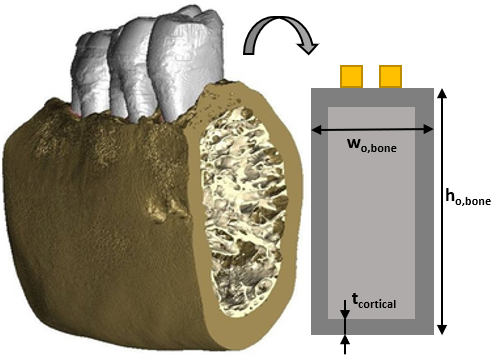
\includegraphics[width=0.7\textwidth]{MandibleCrossSec.png}
    \caption[Cross-sections as used for the beam theory analysis]{Cross-sections as used for the beam theory analysis. a) Cross-section of the jaw plate (indicated with JP in the figure) around the third hole (arbitrary, break does not always occur around this hole) with indication of height ($h_{JP}$) and width ($w_{JP}$) as they are used in the beam theory equations (merged to one rectangle with height $h_{JP}$ and width $w_{JP}$). b) Cross-section of the mandibular body and approximation of this cross-section with simple geometries. $w_{o,bone}$ and $h_{o,bone}$ are the outer width and height of the cross-section, respectively. $t_{cortical}$ is the thickness of the cortical bone.}
    \label{fig:MandibleCrossSec}
\end{figure}

The stiffness of the cortical and trabecular bone in the fracture area changed over time to capture the bone healing process \cite{Voss}. Two scenarios are possible for cortical bone healing: one with direct contact between the broken bone ends and one without \cite{Marsell}. If the broken ends are pressed against each other and are rigidly fixed in place, direct bone healing occurs. This requires the gap between the bone ends to be smaller than 0.001 mm and the interfragmentary strain to be less than 2\%. Cutting cones, consisting of osteoclasts, cross the fracture line and leave behind cavities, which are later filled by osteoblasts. In this way, the continuity of the bone is restored, along with the Haversian systems in the axial direction. If the gap between the bone ends is larger and relative motion is possible between the bone ends, indirect healing occurs. In this scenario, a number of different tissues (including fibrous tissue and cartilage) are formed between the bone ends over time and the stability of the fracture region is gradually enhanced. In the trabecular bone, osteoblasts deposit new bone in the fracture gap by laying it on the existing bone trabeculae and along the fibers of the fibrous tissue that forms prior to bone formation \cite{Voss}.

In this study, the jaw plate was assumed to be able to sufficiently restrict the relative movement of the bone ends of the mandible with respect to one another for direct bone healing to be the most likely scenario to occur.

Lakatos et al. found the modulus of the trabecular bone in the mandible to range from 6.9 MPa to 199.5 MPa \cite{Lakatos}. The modulus of the trabecular bone after fracture started from 0 MPa and rose linearly, for the sake of simplicity, to a value of 100 MPa over the course of 168 days. The cortical bone around the fracture site was initially immature and had a modulus of around 1 GPa \cite{Isaksson}. This immature bone was replaced by stronger, mature bone with a modulus of around 6 GPa and later by compact bone \cite{hawkeye}. Because the precise rate of stiffening was not reported, a rough estimation was made here increasing the bone modulus to 1.3 GPa over the same time period of 168 days as reported for trabecular bone.

To implement the bone regeneration on the simplified geometry shown in Fig. \ref{fig:MandibleCrossSec}b, beam theory equations were used. Details about these can be found in the appendix. The neutral axis was first calculated with a transformed-section method to take the different materials into account. Then, the area moments of inertia of the different sections were calculated. Finally, the stress in the section that corresponds to the jaw plate was calculated and was converted to a force with the use of integral expressions \cite{beamtheory}. For this, the moment in the mandibular body as a result of the biting force was used. The equations were implemented in MATLAB (MathWorks, USA) and automated to loop over different geometries of the cross-section of the plate and material properties of the bone corresponding to the degradation of the plate and the healing of the bone tissue, respectively.

\newglossaryentry{UTS}{name={UTS},description={ultimate tensile strength}}

Computing the force in the jaw plate as an integral of the stress over the area of the jaw plate relies on stress being a linear function of $y$ (the vertical distance between a point in the cross-section and the neutral axis), meaning that if the neutral axis is within the jaw plate or very close to it, the force may not be very high, while the maximal stress occurring is actually very high. If this stress is higher than ultimate tensile strength (\gls{UTS}), it causes problems that might not necessarily be reflected in the total force. What this also reflects is a situation in which the loading of the jaw plate is not predominantly tensile, but rather bending. Using the force in the jaw plate, as computed by the integral in Eq. \ref{eq:integral}, is only valid if the neutral axis is sufficiently far away from the jaw plate. To check this, the stress variation in the jaw plate and the location of the neutral axis were studied in a sensitivity analysis. The derivation of Eq. \ref{eq:integral} can be found in the appendix. $h_{JP}$ and $w_{JP}$ are the height and the width of the cross-section of the jaw plate, respectively, and $h_{o,bone}$ is the height of the cross-section of the outer (cortical) bone. $E_{JP}$ and $E_{cort.bone}$ are the E-modulus of the jaw plate and the cortical bone, respectively. $E_{trab.bone}$ is implicitly present in this equation due to use the transformed-section method as discussed in section \ref{sec:bonehealing}. $I_{cort.bone}$, $I_{trab.bone}$ and $I_{JP}$ are the area moment of inertia of the cortical bone, trabecular bone and jaw plate, respectively. The formulas for these can also be found in the appendix. $M$ is the moment as a result of the loading and y is the vertical distance from a point in the cross-section to the neutral axis.

\begin{equation}
F_{JP}=\int_{h_{o,bone}}^{h_{o,bone}+h_{JP}} \frac{y \cdot M \cdot E_{JP} \cdot w_{JP}}{E_{cort.bone} \cdot (I_{cort.bone}+I_{trab.bone}+I_{JP})}  \,dy
\label{eq:integral}
\end{equation}

%%%%%%%%%%%%%%

\subsection{Coupling of the models}

The biodegradation simulation results were used to derive the changes in geometry on which both the mechanical characterization and the bone regeneration analyses relied. The output from the mechanical analysis delivered the maximum force that the jaw plate could withstand while the output from the beam theory calculations delivered the actual force occurring in the jaw plate, both as a function of time. The comparison between both values allowed to assess the mechanical behavior of the degrading plate during bone regeneration.

%%%%%%%%%%%%%%%%%%%%%%%%%%%%%%%%RESULTS

\section{Results}
\label{sec:results}

\subsection{Biodegradation results}

The simulation of 120 days of the degradation of the jaw bone plate took 18 hours to run using 170 computing cores. Fig. \ref{fig:results_degradation} shows the visualized interface and magnesium ions release during the corrosion process. It also depicts the mass loss of the bone plate in the \gls{SBF} solution over time as well as the geometries used to perform the mechanical analysis at predefined time points.

\begin{figure}[t]
\centering
\medskip
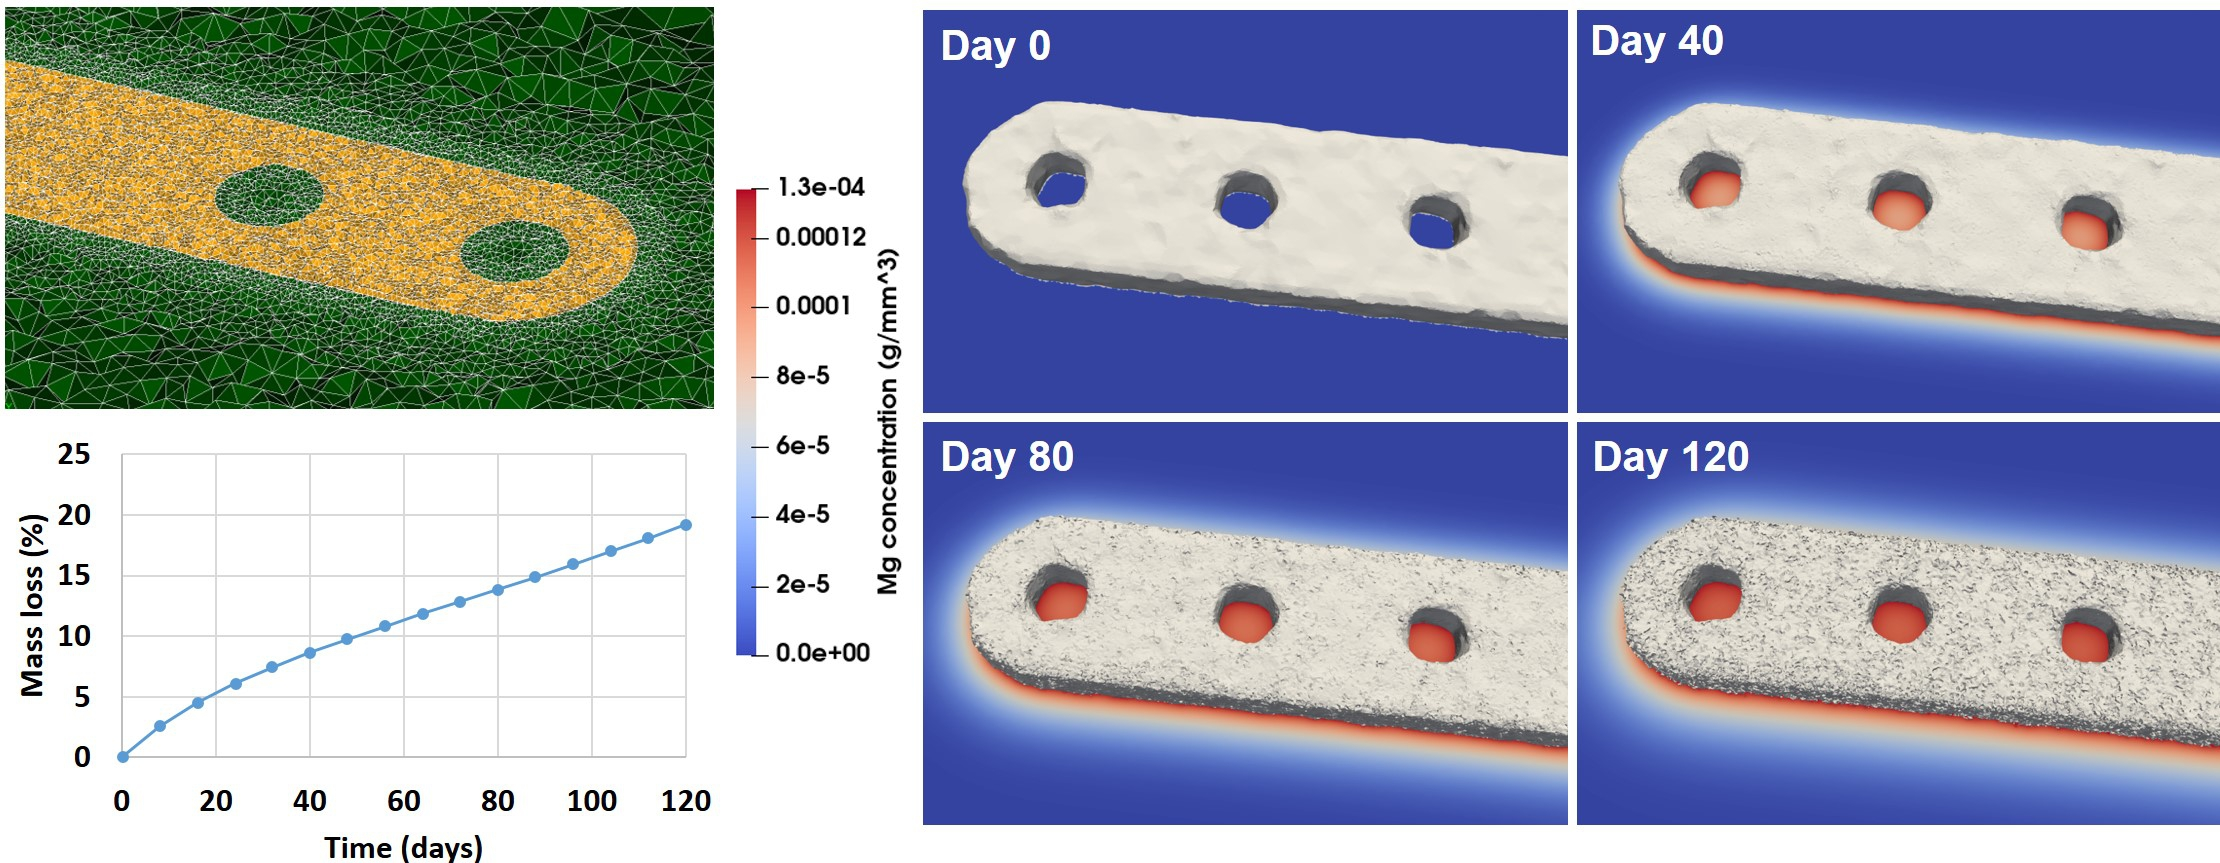
\includegraphics[width=13cm]{results_degradation.jpg}
\caption[Simulation results of the degradation model of the jaw bone plate]{Simulation results. (a) A cross-section of the computational mesh and simulation results of the degradation model of the jaw bone plate in Simlated Body Fluid solution as well as (b) the mass loss graph over time. (c) Degradation of the plate over time. The contours display the concentration of magnesium ions on a cross-section view of the medium beside the moving surface of the bone plate at days 1, 40, 80 and 120. The gray surface is the zero iso-contour of the Level Set function, which corresponds to the surface of the bone plate.} \label{fig:results_degradation}
\end{figure}

%%%%%%%%%%%%

\subsection{Sensitivity analyses}

All models for the tensile tests had a mesh size chosen to ensure presence of four elements fitting into the depth of the plate. The relative difference between the maximal force for four elements compared to five elements fitting into the plate’s depth was only 3.4\%. The computation time for four elements scenario was over 4 hours already and further refining the mesh increased the computation time to over 7 hours. So, in this study, the accuracy gained by refining the mesh did not justify the increase in computation time.

The results from the sensitivity analyses showed that the mass scaling and the use of multiple processors for computation had no impact on the force-displacement curves. The maximum degradation (the point at which an element is removed from the analysis as its load-bearing capacities have diminished due to plastic deformation) only caused changes in the force-displacement curve after the maximum force had been reached, and hence did not impact the maximum bearable force. The displacement at failure and the mesh size, however, did have a strong impact on the resulting force-displacement curves. The maximum bearable force was drastically increased with an increased value of the displacement at failure. Changing the mesh size (i.e. size of the mesh elements) led to the opposite behavior: the maximum force was lower with a larger value of the mesh size. The relationship between both was identified and the numerical misbehavior could be eliminated by adjusting the displacement at failure to the mesh size according to the following general relationship:

\begin{equation}
X_{DAF}=0.6^{log_{0.5}(X_{mesh})}
\end{equation}

\noindent $X_{DAF}$ is the factor with which the \gls{DAF} value should be multiplied when the global mesh size is multiplied with $X_{mesh}$.

The location of the neutral axis was analyzed for the base-line set-up (five-screws) as a representative model for all simulated set-ups in this study. The difference in stress between the top and bottom of the jaw plate was the largest at day 0 and had a value 22.4 MPa at most, which is only 11.6\% of the maximal stress value in the jaw plate and therefore the presence of bending can be disregarded.

%%%%%%%%%%%

\subsection{Coupled models results}

\begin{figure}[h]
    \centering
    \medskip
    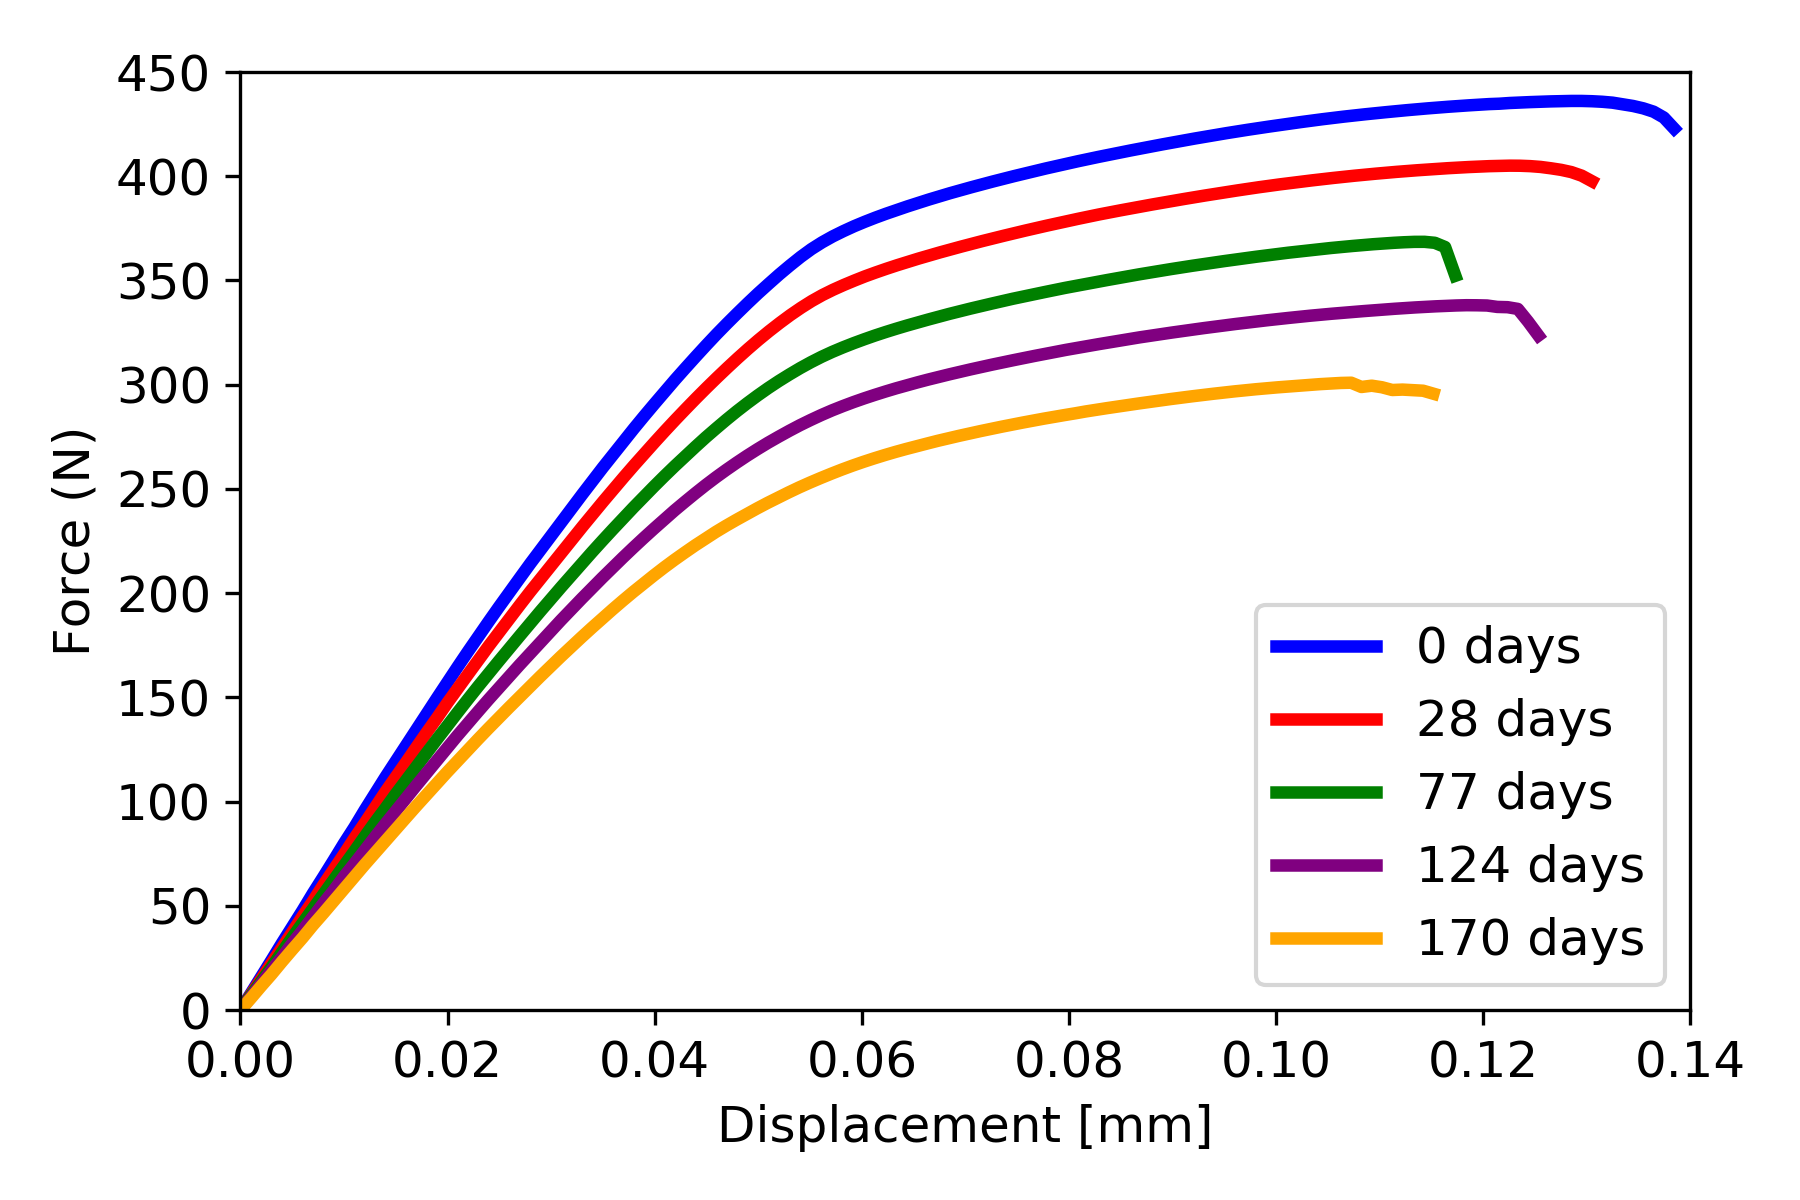
\includegraphics[width=0.8\textwidth]{force_displacement.png}
    \caption{Results of tensile test on jaw plate with five screws with different amounts of corrosion}
    \label{fig:forcedisp}
\end{figure}

\begin{figure}[h]
    \centering
    \medskip
    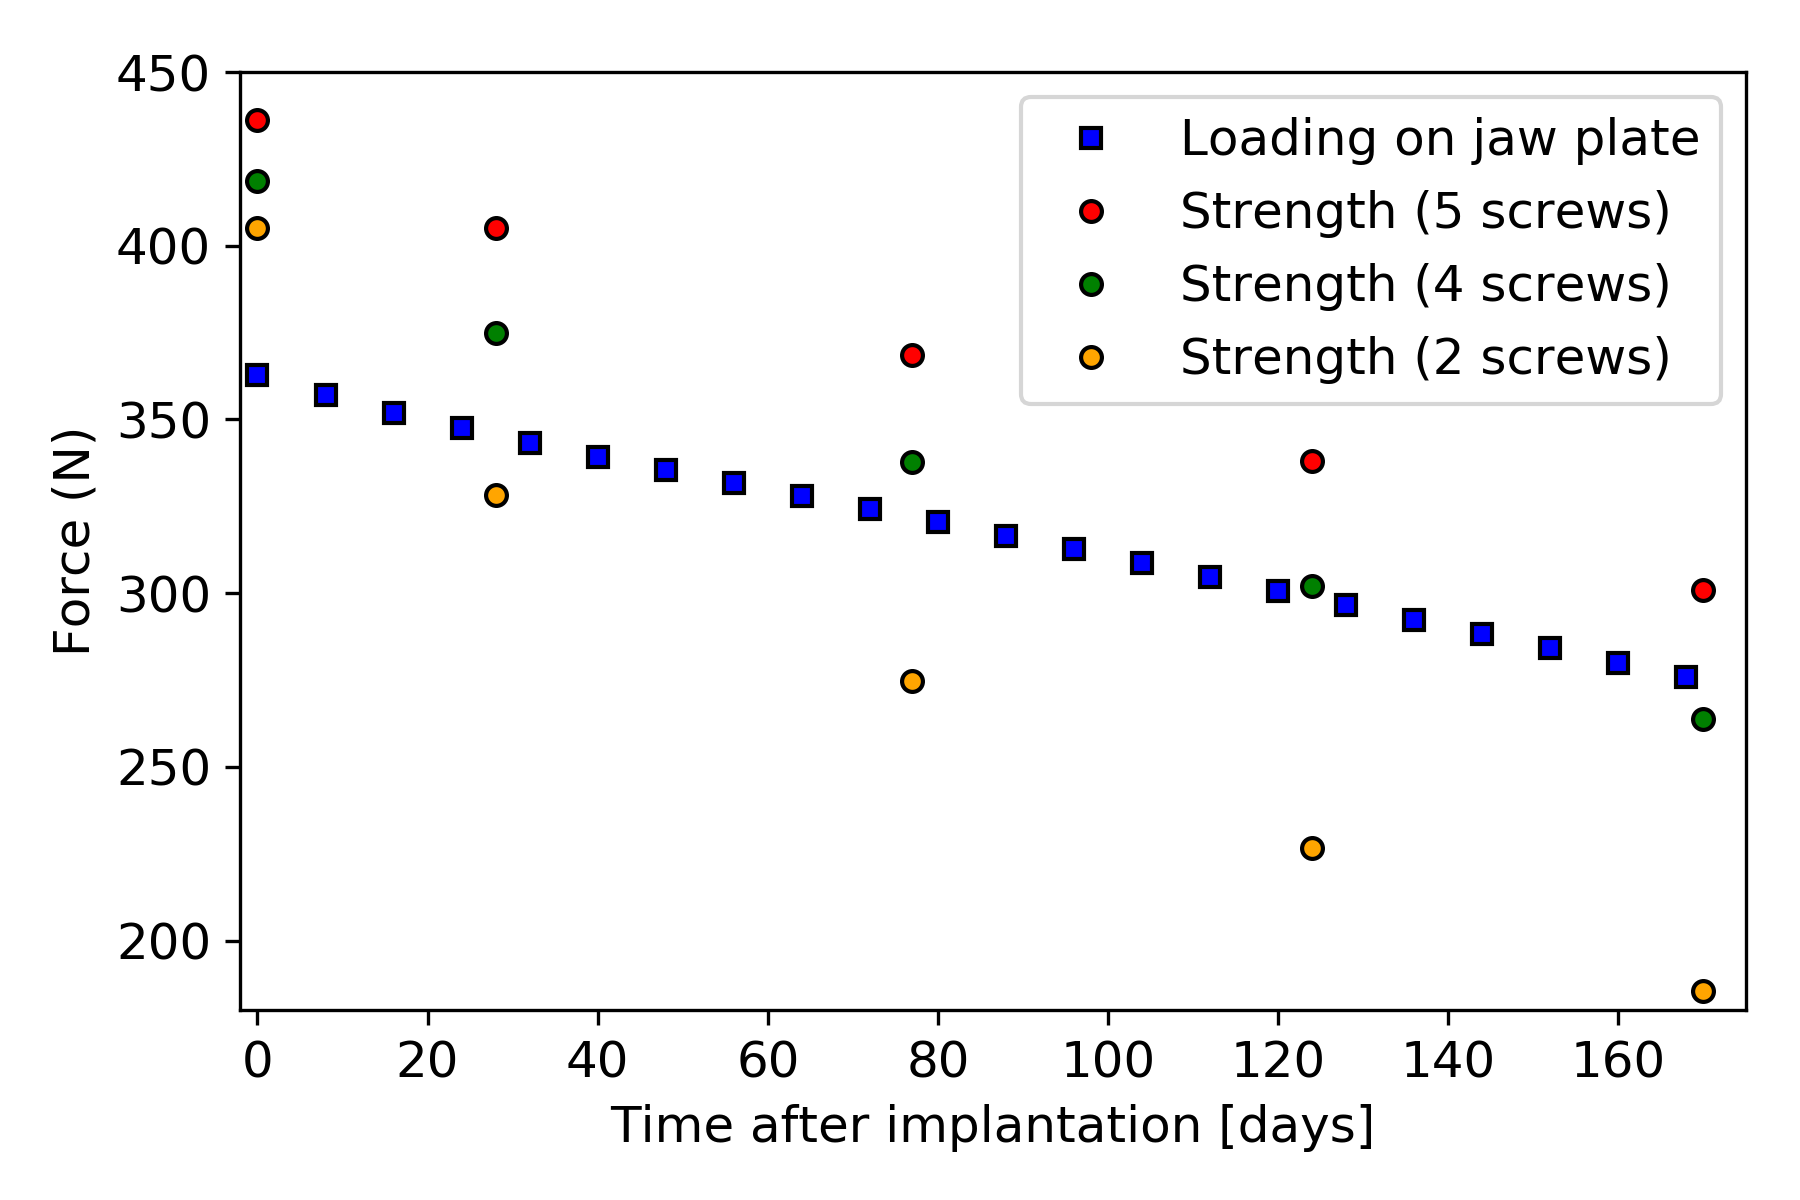
\includegraphics[width=0.8\textwidth]{force_time.png}
    \caption[Estimation of load occurrence as a function of time after implantation for five-screw set-up]{Estimation of load occurrence as a function of time after implantation (days) for five-screw set-up. Maximal force that can be carried by the jaw plate in the different set-ups modeled in this study (same plate, fixed with 5, 4 or 2 screws) calculated at days 28, 77, 124 and 170.}
    \label{fig:forcetime}
\end{figure}

The force-displacement curves for the plate with five screws are shown in Fig. \ref{fig:forcedisp}, with the cases with four and two screws giving similar force-displacement curves. The strength of the jaw plates was characterized by the maximal values from the force-displacement curves. In Fig. \ref{fig:forcetime}, the strength-curves of the jaw plate for the three cases are shown and compared to the loading on the jaw plate, as calculated with beam theory. Comparing the three strength-curves, it could be concluded that leaving more holes open led to a weaker part initially and a faster deterioration of the strength over time as a result of corrosion. In the five-screw case, the strength remained higher than the loading for the simulated time period and hence no failure occurred. In the four- and two-screw cases, failure did occur after about 170 and 20 days respectively.

%%%%%%%%%%%%%%%%%%%%%%%%%%%%%%%%DISCUSSION

\section{Discussion}

In this work, a coupled mechanical-degradation model was presented to study the effect of biodegradation on the mechanical stability of implants for biodegradable mandibular plates. Three different cases were considered, with each a different number of implant holes left unscrewed. One aspect of the difference between the three cases is the surface that was exposed to body fluids as in the cases with fewer screws the open screw holes were also exposed to body fluids. The corrosion inside the open screw holes had an impact on the overall implant strength, as shown in Fig. \ref{fig:forcetime}. Additionally, the boundary conditions representing the screws pulling on the jaw plate are responsible for the differences in the maximal force observed at day 0 since the jaw plate geometry was the same at this point in time for all three cases.

The use of a ``universal'' jaw plate with multiple holes allows the jaw plate to be used in various situations involving mandible fractures. Depending on the exact location of fracture lines and the presence of stronger and weaker sections of bone, the amount and placement of screws can be decided upon by the surgeon. The downside to this is that the differences in mechanical behavior and the change thereof as a result of corrosion between the different cases (5/4/2 screws) can lead to unexpected results if not anticipated correctly by the jaw plate designer and the surgeon. The insertion of screws close to the fracture line was found to be an independent predictive risk factor for implant breakage \cite{Lv2017}. Plates with additional (unused) holes were also found to have an increased risk of breakage. A patient-specific jaw plate can be designed to meet a specific mechanical behavior. As proposed by Lv et al. \cite{Lv2017}, plates should be designed without holes close to the fracture line. The placement of holes can then be a design element for obtaining the desired mechanical behavior of the jaw plate (over time).

The results of the strength simulations provided useful knowledge about the limits in terms of the mechanical strength of the jaw plate and how that evolved during the biodegradation process. Matched with an accurate characterization of the loading, the point at which the jaw plate fails could be predicted. The loading on the jaw plate was derived from the maximal biting force during eating with plate failure occurring if this maximal biting force would be exerted after the point at which the strength curve falls below the loading curve. In practice, the strength of the jaw plate and the way in which this evolves during the biodegradation process are influenced by a range of parameters. Most of these are related to the situation/patient: mandible dimensions, bone properties, fracture line geometry, etc. Others are, however, free to be chosen by the implant designer: the jaw plate material and geometry, the location, the number of screws, etc. Certain restrictions on what food may be eaten by the patient for a certain time period can be given to reduce the maximal biting force and preventive measures should be implemented to avoid bruxism during this period. 

While looking at the relative change in force values led to interesting conclusions, the absolute values of the results obtained in this study were not validated. Manufacturing real samples, immersing them in \gls{SBF}, and objecting them to a tensile test would give \textit{in vitro} results that can be compared to the simulation predictions. However, the obtained results can be effectively compared with similar studies in this regard. An example of such a study is the Imwinkelried et al. work \cite{Imwinkelried2020}, in which they investigated the biodegradation behavior of various designs of mandibular plates \textit{in vivo}, implanted in miniature pig models in multiple implantation sites. Although the design dimensions and number of screws were slightly different from the ones in the current study, the results and conclusion are comparable. In the performed \textit{in vivo} investigations for a rectangular plate inside a tissue pocket in the absence of mechanical load, an estimated total amount of 15\% mass loss was observed within 24 weeks, the value of which is 25\% in the current study (Table \ref{tab:BPdim}). This difference is still reasonable due to the presence of a coating layer and alloying elements in the mentioned study. Moreover, the reported reduction in the bending strength for the mandibular plates is 20\% after 12 weeks, which is in good agreement with the obtained tensile strength in the current study, being 16\% and 19\% for the 5-screw and 4-screw cases, respectively (Fig. \ref{fig:forcetime}).

Another interesting finding of the study performed by Imwinkelried et al. \cite{Imwinkelried2020} is related to the uniformity of biodegradation. According to their findings, in animal studies, the biodegradation of WE43 implants occurred uniformly in the majority of cases, and the implantation site appeared to have little effect on the process based on the selected model. The results indicated that neither the contact between the plate and screw nor the plastic deformation during the implantation process caused localized corrosion of the tested alloy. Moreover, although the presence of a coating layer delayed degradation, it did not significantly alter the underlying behavior of the alloy during degradation. This shows the applicability of the employed computational biodegradation model in the current study, where the effect of non-uniform corrosion was not taken into account for the sake of simplification on the mathematical model. However, the effect of the alloying elements and the coating can be represented by tuning the effective parameters of the model elaborated in \cite{Barzegari2021} and Chapter \ref{ch:core}.

This study has some limitations. First of, the separate analysis of mechanical behavior of and loading on the implant are simplified compared to a structural mechanics model of the entire mandible with jaw plate. This would more accurately capture the loading on the bone-implant complex, including loading modes that deviate from the purely tensile loading as assumed in this study. Second, the results from the biodegradation simulation were simplified to geometry changes based on mass loss data, instead of on its direct output. Finally, the bone healing algorithm was also simplified to linear increases in E-modulus of the bone in the fracture area, which can be developed further to include more sophisticated tissue growth behavior.

\begin{subappendices}

\section{Converting mass loss to jaw plate dimensions}
\label{sec:jawplatedimensions}

The changes in dimensions were assumed to be determined by a 'thickness' of the entire outer surface that was removed as a result of corrosion. If this 'thickness' is represented by $x$, the dimensions of the jaw plate are written as:

\begin{equation}
depth=0.001-2x
\label{eq:depth}
\end{equation}
\begin{equation}
H=0.004-2x
\end{equation}
\begin{equation}
R_i=0.001
\end{equation}
\begin{equation}
R_o=0.002-x
\end{equation}

\noindent Note that $R_i$ was constant, which means that these equations were for the five-screw case. The five-screw case was the reference for the mass loss data from the degradation simulation. So, the change in geometry was calculated for the five-screw case, but could then be applied to all three cases. The volume of the jaw plate was calculated as:

\begin{equation}
Volume=(TH-5\pi R_i^2+\pi R_o^2)\cdot depth
\end{equation}

\noindent with $T$ the length of the straight edge of the jaw plate ($T=L-2R_o$). The value of the mass loss was converted to a volume with the formula:

\begin{equation}
Volume=InitialVolume\cdot  \frac{100-MassLoss(\%)}{100}
\label{eq:massloss}
\end{equation}

\noindent with $InitialVolume$ being the volume for $x=0$. The combination of equations \ref{eq:depth} to \ref{eq:massloss} lead to an equation with two unknowns, being $x$ and $MassLoss$. By solving this equation to $x$ and filling in values of the mass loss, the corresponding values of $x$ were calculated.

\section{Beam theory equations}
\label{sec:beamtheory}

\noindent The formulas in this appendix were based on the book 'Advanced Mechanics of Materials and Applied Elasticity' by Ugural and Fenster \cite{beamtheory}. The mandibular body behaved as a beam and as a result the moment $M$ in the fracture as a result of the load was given by:

\begin{equation}
M=lever arm\cdot load
\end{equation}

\subsection{Neutral axis}

The neutral axis is an axis in the cross-section where the stress is zero. Taking the loading situation into account, everything above the neutral axis is under positive (tensile) stress and everything below the neutral axis is under negative (compressive) stress. Since the approximation of the cross-section was symmetrical with respect to the vertical line through the center of the cross-section, the neutral axis was horizontal. Because different materials were used, with different E-moduli, an extra step was taken before calculating the neutral axis. The width of the cross-sections of different materials was multiplied with a factor that took the E-modulus of the material into account. The E-modulus of the cortical bone was taken as a reference here. This method is called the transformed-section method. $h_{o,bone}$ and $w_{o,bone}$ indicated the height and width of the cortical (outer) bone and $t_{cortical}$ indicated the thickness of the cortical bone layer. $h_{i,bone}$ and $w_{i,bone}$ indicated the height and width of the trabecular (inner) bone and are calculated based on the outer dimensions of the bone and the thickness of the cortical bone layer:

\begin{equation}
h_{i,bone}=h_{o,bone}-2t_{cortical}
\end{equation}
\begin{equation}
w_{i,bone}=w_{o,bone}-2t_{cortical}
\end{equation}

\noindent The relevant dimensions of the jaw plate (abbreviated as JP) cross-section were the height ($h_{JP}$) and the width ($h_{JP}$). The two individual rectangles were treated as one, since this made no difference in the calculations. As mentioned above, the widths of the trabecular bone and the jaw plate were adjusted:

\begin{equation}
w'_{i,bone}=w_{i,bone}\cdot \frac{E_{trab.bone}}{E_{cort.bone}}
\end{equation}
\begin{equation}
w'_{JP}=w_{JP}\cdot \frac{E_{JP}}{E_{cort.bone}}
\end{equation}

\noindent The areas of the trabecular bone, cortical bone and jaw plate, as used for the calculation of the neutral axis, were:

\begin{equation}
A_{cort.bone}=h_{o,bone}w_{o,bone}-h_{i,bone}w_{i,bone}
\end{equation}
\begin{equation}
A_{trab.bone}=h_{i,bone}w'_{i,bone}
\end{equation}
\begin{equation}
A_{JP}=h_{JP}w'_{JP}
\end{equation}

\noindent The accented widths were the E-modulus-adjusted widths. The height of the neutral axis with respect to the lowest point of the bone cross-section was calculated as:

\begin{equation}
y_{mid}=\frac{A_{trab.bone}y_{trab.bone}+A_{cort.bone}y_{cort.bone}+A_{JP}y_{JP}}{A_{trab.bone}+A_{cort.bone}+A_{JP}}
\end{equation}

\noindent with $y_{trab.bone}$,$y_{cort.bone}$ and $y_{JP}$ the height of the center of mass of the different sections, which were (relative to the lowest point of the bone cross-section):

\begin{equation}
y_{cort.bone}=y_{trab.bone}=h_{o,bone}/2
\end{equation}
\begin{equation}
y_{JP}=h_{o,bone}+h_{JP}/2
\end{equation}

\subsection{Area moment of inertia}

The area moment of inertia of the different materials in the cross-section were calculated with equations \ref{eq:i1} to \ref{eq:i2}. The total area moment of inertia was the sum of those (equation \ref{eq:i3}).

\begin{equation}
\label{eq:i1}
I_{cort.bone}=\frac{w_{o,bone}h_{o,bone}^3}{12}-\frac{w_{i,bone}h_{i,bone}^3}{12}+(y_{mid}-y_{cort.bone})^2\cdot A_{cort.bone}
\end{equation}
\begin{equation}
I_{trab.bone}=\frac{w'_{i,bone}h_{i,bone}^3}{12}+(y_{mid}-y_{trab.bone})^2\cdot A_{trab.bone}
\end{equation}
\begin{equation}
\label{eq:i2}
I_{JP}=\frac{w'_{JP}h_{JP}^3}{12}+(y_{mid}-y_{JP})^2\cdot A_{JP}
\end{equation}

\begin{equation}
\label{eq:i3}
I=I_{cort.bone}+I_{trab.bone}+I_{JP}
\end{equation}

\subsection{Stress, strain and force}

The moment that was created by the load caused the beam to bend and this induced stresses in the cross-section. The radius of curvature $\rho$ was first calculated and used to calculate the strain $\epsilon$. For that, the distance with respect to the neutral axis $y$ was also used.
\begin{equation}
\rho =-\frac{E_{cort.bone}I}{M}
\end{equation}

\begin{equation}
\epsilon =-\frac{y}{\rho}
\end{equation}

\noindent The strain depended on $y$, but there is no difference between different materials. When calculating the stress $\sigma$, however, the incorporation of the E-modulus did make a distinction between the different materials. The stress in the jaw plate was:

\begin{equation}
\sigma _{JP} =\epsilon \cdot E_{JP}
\label{eq:stress}
\end{equation}

\noindent Finally, the stress in the jaw plate was integrated over the area of the jaw plate to find the total force in the jaw plate:

\begin{equation}
F_{JP}=\int_{h_{o,bone}}^{h_{o,bone}+h_{JP}} \sigma _{JP}\cdot w_{JP} \,dy
\end{equation}

\noindent It was important to use $w_{JP}$ here, which represented the non-adjusted width of the jaw plate, since the calculation of the stress in equation \ref{eq:stress} used the E-modulus of the jaw plate.


\end{subappendices}


%%%%%%%%%%%%%%%%%%%%%%%%%%%%%%%%%%%%%%%%%%%%%%%%%%
% Keep the following \cleardoublepage at the end of this file,
% otherwise \includeonly includes empty pages.
\cleardoublepage
